% This example An LaTeX document showing how to use the l3proj class to
% write your report. Use pdflatex and bibtex to process the file, creating 
% a PDF file as output (there is no need to use dvips when using pdflatex).

% Modified 

\documentclass{l3proj}
\begin{document}
\title{Team V - How Not To Kill Your Dog}
\author{Ross Adam \\
        Andrew Gardner \\
        Nicole Kearns \\
        Mamas Nicolaou \\
        Asset Sarsengaliyev}
\date{18 March 2013}
\maketitle
\begin{abstract}

The abstract goes here

\end{abstract}
\educationalconsent
\tableofcontents

\chapter{Implementation}
\label{implementation}
\section{Abstract}
\section{Developing a Web Based Application }
One of the requirements for our project was that our final product should be available to 
use to any user with an Internet Connection. More specifically, any student should be 
able to access the application and practice on their drug calculations in their free time 
wherever they are with any device that can access the Web. This can be a laptop 
computer, a mobile phone or a tablet computer. \\ 
It was, therefore, clear to us that creating an application that needs to be installed on a 
machine in order to be usable was not an option. After a discussion with the team we 
decided that the most suitable solution would be to implement a application that would be 
accessible via a Web Browser. A web application would make it possible for any user to 
access our application from any device simply by navigating to our Web Applications 
URL address. \\ 

\subsection {Using a Web Application Framework}
After doing some research looking for the best possible option for developing web 
applications we decided that we would make use of a web development framework 
rather than writing the code for the whole application from scratch.
\subsubsection{ Developing from Scratch}
Developing an application from scratch has the potential to take up much needed time 
from the Development Phase. For each different page of an application there needs to be 
a unique file (for example an html document) that will be sent to the client's web browser 
when the page is called. An application usually has the same layout on every page with 
basic components, like the applications logo or the applications default buttons, being 
displayed on each page. It is therefore clear that having a separate file to correspond to 
each different page of an application can lead to a lot of coding overhead and 'boiler 
plate' code. In the case of a change request, a developer will need to modify the code in 
each different page separately which would take much of our development time. Time was a major concern for us as we only had a limited amount of time to get the application designed, developed, evaluated and delivered to our client.
\subsubsection{Developing with a web application framework}
A Web Application Framework is a set of prefabricated software building blocks that 
programmers can use, extend, or customise for specific computing solutions" (Leif 
Azzoperdi, DIM3 Lecture 3). A framework would allow us to start implementing our 
application with a concrete base to support us by providing default functionality whilst 
allowing us to extend or override functionality to suit our specific requirements. "One 
significant advantage to using a framework is that you're required to write only a 
minimal amount of code to get up and running from scratch"(Professional Python 
Frameworks: Web 2.0 Programming with Django and Turbogears page 48). This was 
one of the most important reasons for which we opted in using a Web Application 
Framework for our project. Afterwards, there was one more decision that needed to be 
undertaken. There are a number of frameworks available on the web so we had to decide 
on one of them before starting our implementation. 
\subsection {Which framework to use?}
We came down to three popular web application frameworks that would help us develop 
our software but we had to decide on one of them. Our supervisor suggested that three 
of us take one of the three frameworks each and try to build a simple application in one 
week. This would not only show us what can be built with that particular framework but 
it would also show us how long it take for a developer to learn how to use the 
framework, and how much can be built in a week by using that framework. The three 
options were 
\begin{itemize}
\item Web2Py 
\item Django 
\item Ruby on Rails 
\end{itemize}
After our frameworks evaluation we came to the following conclusions about them: 
Ruby on Rails offers useful code generators which can produce functions out of one line 
of code written by the developer and has a build in testing framework which can be 
particularly useful for our testing. However, the mystery behind the code generators can 
cause confusion to developers and thus increase development time. \\
Web2Py uses a Python-based template language and supports development from a Web 
Browser. We have been using python for our introduction to programming course in Level 
1 of our university studies so it would python is a language we have all used and are 
comfortable with. Moreover, a developer needs not have their own computer with them 
to work on the development of the application. Web2Py gives the ability to a developer 
to work on the code of the application via a web interface which can be particularly 
useful in case one of the team members is traveling and is not able to use their own 
computer to work on application. \\
Django is an MVT (Model, View, Template) based framework that runs with Python on 
its back end. This gives us the advantage of having separation of concerns in our 
application since different components in the framework act independently from each 
other so a developer can work on one part of the application while another can work on 
a different component without having to wait for a different component to be completed. 
Django is an extremely customisable framework since it comes packed with a lot of 
functionality which can be used out of the box or can be further modified to reflect our 
goals and objectives. On the other hand it might take time to learn since it has its own 
way of doing things and a developer needs to adapt to it.

\subsection {Why Django}
We decided to use Django since it gives us great flexibility as to what our end product 
can be like, it is documented extremely well online and even though learning it can take 
some time, we consider it to be a well worth investment since we will have to use 
Django in one of our courses in second semester as well. 
\section{Development in Django}
As its being described on djangoproject.org, Django is "The Web framework for 
perfectionists with deadlines". It is a rapid web development framework that can save 
you the trouble of writing repetitive boilerplate code. A developer using Django can 
achieve greatness with minimal coding. Django comes with an object relational mapper 
which means that we can define our database schema in Python code by defining 
classes and Django will then produce an sql code that can be injected in our database 
with minimal effort from the developer in order to create any tables required for the 
project. It has a dynamic build in administration interface which can be customised 
according to our needs. This can be used, in our case, as a way for a Course 
Coordinator or a Tutor to create new topics, add slides and questions to each topic, 
create questions for the final assessment page and create new users or groups of users 
with special permissions. This will be discussed further in this report.
\subsection{The MTV Model}
The MTV model used by django is a development mode very similar to the MVC model which is widely used by a number of web application 
frameworks such as Backbone.js SproutCore and the Cocoa framework used in Mac OS X and iOS applications. Django, since it likes to do things its own way, uses a "modified" version of the MVC model. Its model is called MTV (Model, Template, View). The model in the MVC 
plays the same role as the model in MTV which is sensible. However, the "View" in the 
MTV maps to the "Controller" of the MVC and the "Template" of the MTV maps to the 
MVC's "View". Of course this is slightly complicated so it might cause some confusion to 
a developer coming from an MVC background. 
The MTV in general defines the way everything works in Django. Everything in Django 
can be broken down to 3 components; The Models, the Templates and the Views.
\subsection{Models}
"A model is the single, definitive source of data about your data. It contains the essential 
fields and behaviours of the data you are storing"(Django website). In other words, any a 
table in the database can be created by defining a model in the Models.py file. A 
database field for that table can be defined as an attribute of the corresponding model. 
The command "manage.py syncdb" will then read the Models.py file create an SQL code 
and then run it agains the applications database to create any tables defined by the 
developer. 
For example if the code in picture below is run it will create a Database table of topics 
where each topic has a title and a publication date. \\
class Topic(models.Model): \\
title = models.CharField(max\_length=100) \\
pub\_date = models.DateTimeField('Date Published')\\
\subsection{Views}
A view takes care of what is sent to a browser when a specific URL is requested. It is 
responsible for making any requested action as this is defined in the tags of the html 
page associated with each view. Such actions might be read or write to the database 
commands or any other actions that are required by a page.
\subsection{Templates}
A template is usually an html file. It is the base of what will be send on to a web browser 
client. It described how the data should be presented to the user and can contain a 
number of Django tags and variables. A tag is surrounded by "" and tells 
Django that a special action needs to be taken at that point of the page. This special 
action can be an "if" statement, a "for" loop etc. A variable is simply telling Django to load 
a specific value from the Database and display it at this point of the page. Templates are 
used by Django as the model for a page to be sent to a web client.
\subsection{Controller}
Each Django application has a "urls.py" file which holds definitions that will be matched 
against requests by web clients. An example url definition in "urls.py" could be \\
\verb|"url(r ^'contents', 'views.contents')"|. \\In this scenario if our server is hosted on 127.0.0.1 
port 8000 and a client requests "127.0.0.1:8000/contents" Django will match the 
request with the definition in "urls.py" and call the appropriate view which is the second 
argument of the url() function. In this case it will be the "contents" view.
\section{3-Tier Architecture}
For our implementation we used a 3-Tier Architecture.
\subsection{N-Tier Architecture Diagram}
 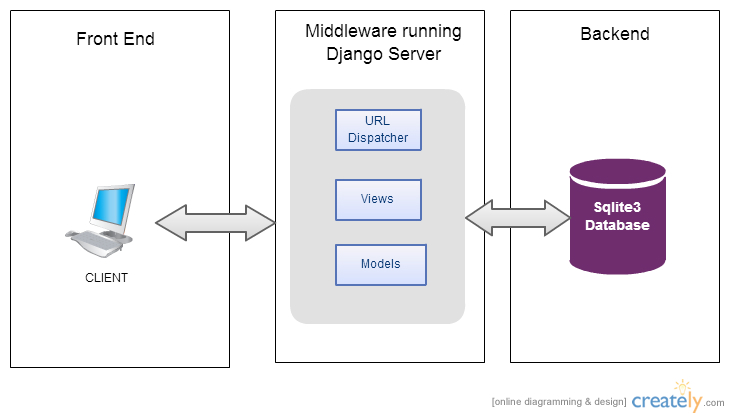
\includegraphics[width=\linewidth]{images/ntier.jpg}
\subsection{Front End}
The application can be accessed by any user with a web browser such as Internet 
Explorer, Google Chrome, Mozzila Firefox, Safari and so on. \\
\subsection{Middleware}
This is our Django server. Responsible for matching requests from Clients using the 
URL dispatcher which in return calls the appropriate View which then fetches any 
required context from the Models.py and our Backend Services. 
\subsection{Back End}
This is our Sqlite3 Database. Other database options included MySQL, Oracle or 
PostgreSQL. However we opted in for Sqlite3 since it offers all the functionality we 
need and Django provides more support for it as it is its default option. \\
\section{Back End - Data Models}
Our database consists of 4 basic data models. 
\subsection{Data Model:Topic}
\begin{tabular}{|c|c|c|}
\hline \textbf{Field Name} & \textbf{Type} & \textbf{Notes}\\
\hline title & CharField & 1000 characters max \\ 
\hline pub\_date & DateTime &  \\ \hline
\end{tabular}
\subsection{Data Model:Question}
\begin{tabular}{|c|c|c|}
\hline \textbf{Field Name} & \textbf{Type} & \textbf{Notes}\\
\hline qTopic & ForeignKey & Points to a Topic object \\ 
\hline text & CharField & 1500 characters max \\
\hline answer & CharField & 100 characters max \\ \hline
\end{tabular}

\subsection{Data Model:FinalTestQuestion}
\begin{tabular}{|c|c|c|}
\hline \textbf{Field Name} & \textbf{Type} & \textbf{Notes}\\
\hline text & CharField & 2000 Characters max length \\ 
\hline answer & CharField & 100 characters max \\ \hline
\end{tabular}

\subsection{Data Model:Slide}
\begin{tabular}{|c|c|c|}
\hline \textbf{Field Name} & \textbf{Type} & \textbf{Notes}\\
\hline sTopic & ForeignKey & Points to a Topic object \\ 
\hline image & ImageField &  \\ \hline
\end{tabular}

\section{Managing the Front End}
The way Django is generally managing the Front End of an application is quite 
straight forward. It simply takes a predefined template (html file), adds any required 
content from the models (database objects) and sends the file over to a web browser. 
However creating simple html files and feeding them the data from our models is not 
enough to produce a high quality web application. The fact that we were not 
experienced in web application was not helping us find a solution without investing 
some time on researching. In our quest to find a way to manage the front end design 
we looked at a number of solutions. Some of them were the "Backbone.js", "Tastypie" 
and "Pyjamas". At a first glance each of these frameworks seemed promising. 
However, trying to use them to produce high quality front end design became more of 
a time wasting challenge rather that a time worthy investment.
\subsection{Possible frameworks for Front End management}
\subsubsection{Backbone}
As its website states, "Backbone.js gives structure to web applications by providing 
models with key-value binding and custom events, collections with a rich API of 
enumerable functions, views with declarative event handling, and connects it all to 
your existing API over a RESTful JSON interface". Fair enough, now how can we 
proceed and use this Framework with our Django application? A number of github 
repositories were available online, all with example applications using Backbone. 
However, since all of them were out of date and description for Backbone and 
Django integration was vague at best, we soon abandoned the idea of using 
Backbone. 
\subsubsection{Tastypie}
TODO!
\subsubsection{Pyjamas}
Pyjamas is a framework which takes code written in Python and translates that 
into javascript and jquery code without the need of having a developer experienced 
in using javascript and jquery. We managed to get Pyjamas set up successfullly, 
but the result was not exactly what we expected. The design looked poor and we 
had to invest even more time in advancing our skills on coding a GUI with python
\subsubsection{Compination of traditional Django friendly frameworks}
Luckily for us, one of our team members who is really confident on his web design skills
convinced us that surely using traditional web design methods, such as writing the code for the templates directly in javascript and using a simple collection of tools such as the Twitter Bootstrap might be worth looking into. He suggested that he can try work out a first draft of the Topics page so that we can see what he can produce with these tools and judge for ourselves. Creating the page actually took him less than one hour and that was a wakeup call for us since the sample page he created was both looking aesthetically nice and the technologies used were working with the Django seamlessly with minimal effort.  
We started by creating a base.html template. Django gives a developer the option to create templates that inherit from other templates. So any code that needs to be repeated in every page needs not be defined more than once. Our  base page with no additional content can be seen on figure "base.jpg". This includes the basic layout that should be displayed on ALL templates of our application. So to make the connection between our base template and all other template we had to define an empty Django tag  called “content block” in our base.html template. Then on every page that needs to inherit from base.html we can define the content block so that it includes any additional data that each specific template may require. An example of how a block is defined in a base template is shown in figure “baseblock.jpg” and then the way the base template is inherited and the “content block” is used can be seen on figure "extendsbase".
\begin{figure}[h!]
   \caption{A picture of a gull.}
   \centering
     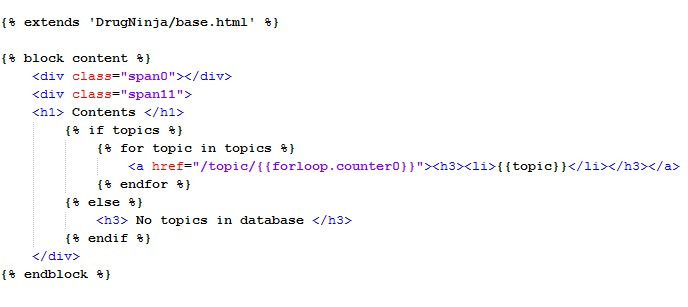
\includegraphics[width=0.5\textwidth]{images/extendsbase.jpg}
\end{figure}
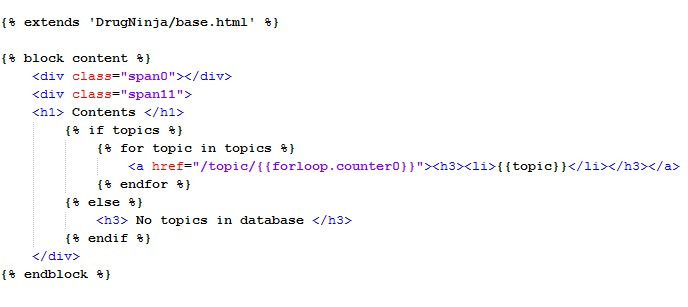
\includegraphics[width=\linewidth]{images/extendsbase.jpg}
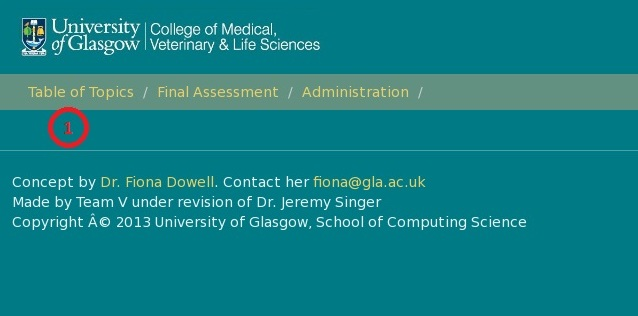
\includegraphics[width=\linewidth]{images/base.jpg}
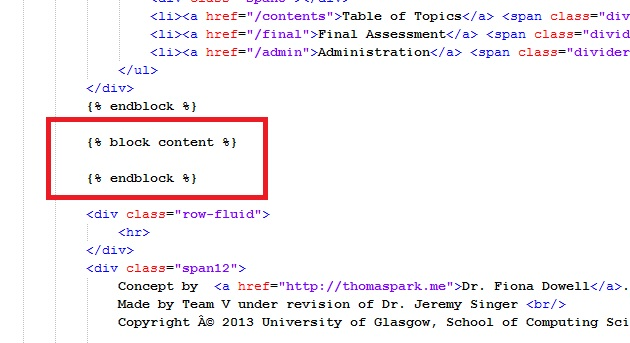
\includegraphics[width=\linewidth]{images/baseblock.jpg}
\section{Middleware: Linking the back with the front}
Django makes the connection between the backend data models and the front end templates by interpreting a request from a web client, finding the required template for that request and rendering the context on the page by replacing all Django tags (text surrounded by '{\%' and  '\%}') with data returned by the responsible view for that request.  For  instance, figure **contentsView** shows how the contents View is defined. The tag “topics” is declared as a list of Topic objects and then by adding the key “topics” into the contents view context we are telling the view to return the list “topics” every time the tag “topics” is found on the template “contents.html”. Then in template “contents.html” we make use of a for loop to iterate through the topics list, and print out the topic name with a link to its unique url. After the template has been rendered it is sent on to the web browser where it is presented to the urer who requested the page.
\section{Message Passing}

\subsection{Database Request Format}
Database Requests are handled by Django. A template may require information about a specific data model. The view that makes use of that specific model makes SQL request to the database which in turn returns any matching results from our SQLite database.
Image **dataMessagePassing.png***

\subsection{Answer Validation Request}
The validation of answers is done by an Ajax request to  the “validateAnswer” view or to the “validateFinalAnswer” view when the answer to be validated belongs to a final assessment type question. The validation is done by passing the question id and the provided answer as URL parameters. The view  then makes a request to the database requesting the answer of the required question. If the answer provided by the user is the same as the one stored in the database the view will respond to the web client with an appropriate Http Response as on figure **validateAnswer figure**. 

\subsection{Topic Related Data Request}
Topic requests make use of the “Topic” view. The view uses the “topic.html” template and renders it so that it gains access to a list of Topic objects. When, for example, a user needs to navigate to the appropriate page for the first topic in the Topic objects list, they should navigate to “/topic/0” where 0 is the position of the first Topic objects in the topics list. When the slides of a specific Topic need to be displayed, a “for” loop is used to iterate through the list of slides and return only those that point to the Topic that was originally requested by the URL.

\section{End Product}
\subsection{Desired Functionality}
The Desired Functionality section aims to describe how the desired functionality mentioned in Requirements and Design sections was realised through the implementation will now be demonstrated in more detail.

\subsubsection{Welcome Page}
The welcome page is implemented through the “index” view.  It is maybe the simplest template in our project. It is a simple template that inherits from base.html and includes a static text with a brief description of our web application and a button that points to the first topic page.
Welcome Page figure

\subsubsection{Topic Page}
The topic page consists of two equal width side bars. The left sidebar is a carousel which displays all the slides related to each topic and the right sidebar  consists of a “for” loop that displays all the questions related to each topic along with a text box for a user to enter their answer and a submit button. Once a submit button is pressed, an ajax call makes a request to the server which responds with a “correct answer” or “false answer” accordingly.  The response from the database updated the string on the submit button so the text on the button changes from “Submit” to “Correct answer” or “False answer”.
Topic page figure

\subsubsection{Contents Page}
The contents page is implemented so that a user can navigate directly to a specific topic page without having to go through all other topics via the “Next” button on each topic page. A “for” loop is used on “contents.html” template which is used so that the “contents” view will replace the contents of the “for” loop with a list of all Topic Names currently stored in the database with links that point to that specific Topic’s page.
***contents figure***

\subsubsection{Final Assessment Page}
The final page is one of the core components of our application. The requirements were clear. A user should be faced with 10 random questions from the “FinalAssessmentQuestion” database model and he or she should only be allowed to have one attempt to answer the question. This is to make sure that a user pays the required amount of thinking before clicking the “Submit Answer” button. Our client initially provided us with a number of sample lecture slides so that we could get an idea of her lectures’ contents. We noticed that a picture she uses often to make her lecture slides more interesting to students is a picture of “donkey” from the Shrek movies. So we thought that since the users are probably already familiar with the Shrek donkey so we added it on a side bar in an attempt to make the Final Assessment Page more interesting and appealing to the users. We also added a “health bar” and a “Score” label. The score label has a maximum value of 100\% and it defaults to 0\% while the “health bar” has a maximum value of 100\% but defaults to the maximum. Each time a user enters a value to a questions text box and clicks the “Submit Answer” button an Ajax request is sent to the Django server which responds with “Correct Answer” or “False Answer”. If the answer was correct, the Score label will be update with the current score + 10 and the health bar will not be modified. However, if the answer was wrong the value of the health bar will go down by 10\% and the score will remain the same.  In addition, if the value of the health bar falls below 50\%, the image of the donkey will change from the default “happy donkey” to a “sad donkey” and then if it falls below 1\% an alert will be displayed to the user with a “You have killed your animal” notification and the picture of the donkey will be changed to a dead donkey.  A colour coded response is also displayed to the user as the question box turns red if the users answer was wrong, or green if the users question was correct. 
Final assessment figure
\subsubsection{Administration Page}
The administrator page is dynamically created by Django. We only needed to define which models needed to be modifiable from the admin page and the  way we want them to be displayed.  Two groups of modifiable data models were defined. “Topics” and “FinalAssessmentQuestions”. The reason behind this was that questions and slides have a foreign key that points to a Topic so by selecting a Topic in the administration page a user can see and modify all slides and questions that are related to that Topic. By navigating to the “FinalAssessmentQuestions” a user can add, delete or modify a Final Assessment Question. By default, Django also provides a user management interface by which  a user with administrative rights can manage users by adding, removing or modifying permissions for other users.
**figure admin interface**

\subsection{Interaction Diagrams}
\subsubsection{Topic Page}
\begin{figure}[!htb]
\caption{Topic Page Interaction Diagram}
 \centering
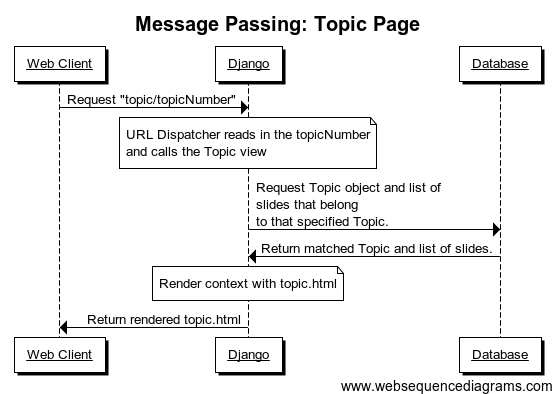
\includegraphics[width=0.9\textwidth]{images/topicPageMessagePassing.png}
\end{figure}

\subsubsection{Contents Page}
Interaction diagram for communications and message passing between the Contents Page and the server
\begin{figure}[!htb]
\caption{Contents Interaction Diagram}
 \centering
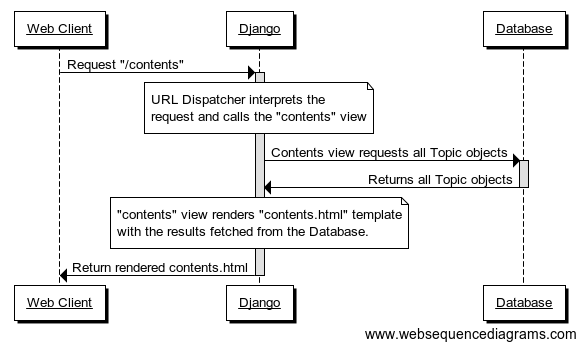
\includegraphics[width=0.9\textwidth]{images/contentsInteractionDiagram.png}
\end{figure}
\subsubsection{Final Assessment Page}
Interaction diagram for communications and message passing between the Final Assessment Page and the server
\begin{figure}[!htb]
\caption{Final Assessment Interaction Diagram}
 \centering
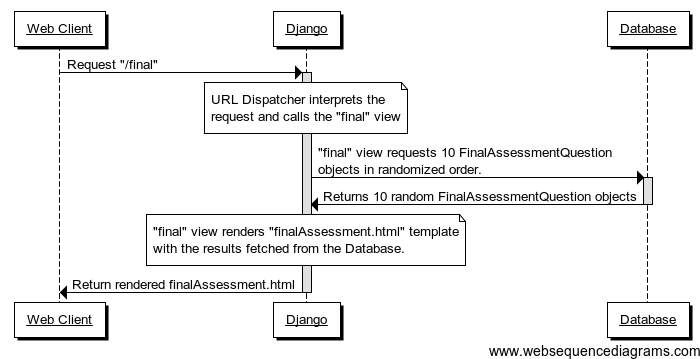
\includegraphics[width=0.9\textwidth]{images/finalAssessmentInteractionDiagram.png}
\end{figure}
\section{Challenges and Solutions}
Referencing topics by topic.id
When we first started working with topics we were using the topic ids provided by Django to reference and call topics from a template's perspective. However we soon realised that Django was using the IDs provided by SQL and not some IDs that were generated by Django. The result of this error on our behalf was that when a Topic was removed from the database, the ID numbers for topics were not automatically regenerated so clicking the next button (this calls topic with topic ID equal to the current topic's ID+1) on a Topic page would call a Topic ID that might not exist in the database. Consequently, that would cause the application to run on an Index error In order to bypass this issue, we looked at alternative ways of indexing the list of Topics and returning available Topic numbers.  Instead of using Topic IDs we started using Topic List positions. More specifically, we are now creating a list of Topics in Topic view by requesting ALL the Topics currently held in the Database and then iterate over that one. For example, when “/topic/0” is called, instead of requesting Topic with TopicID==0 from the database, we are requesting the Topic in position [0] of our runtime created Topic list. This way, the numbers used to request topics are always up to date with exactly what's currently held in the Database.  We have also added checks to see whether the current topic is the first or last topic in the Topics list. In which case the “Next” or “Previous” buttons are hidden accordingly.

URL Dispatcher for Validating Questions
As mentioned in previous sections, the way we validate answers is by passing them as parameters with an Ajax Request.  The URL dispatcher then matches the url the web client requests and matches that with the “validate” url definition in urls.py. The url definition for “validate_answer” is: “url(r'^validate_answer/(?P<question>\w+)/(?P<answer>\w+)', 'views.validate')”. By definition (?P<answer>\w+) accepts any string as answer. However when a user provides an answer such as “2.5”, the URL dispatcher accepts “2” and disgards anything after the decimal point. This was causing answer validations to fail even when the answer provided by the user was correct. The Django documentation on URLs was not particularly helpful so through a process of trial and error we arrived at a valid solution that can match both strings (this can be a non decimal number as well) and decimal numbers. In addition to our “url(r'^validate_answer/(?P<question>\w+)/(?P<answer>\w+)', 'views.validate')” regular expression we added “url(r'^validate_answer/(?P<question>\w+)/(?P<answer>\d+\.\d+)', 'DrugNinja.views.validate')” right before the first expression. In essense, when a validate answer request arrives, the URL dispatcher will try and match it to the new reqular expression which only matches answers with a decimal point. If the answer does not match, Django will try to match it to the second URL definition which accepts strings or non decimal integers and respond accordingly.
Static Files
Django has some strict safety rules when it comes to static files. When we started our implementation, having only basic web design knowledge, we though that defining a static files directory would be enough for Django to be able to write and read files. This seemed to be the case since when we were uploading images to the system through the administration interface, the system seemed to be reading the files just fine and saving them in the correct directory. However, when a web browser made a request for a static file Django was returning 404 errors referring to a local file that we were sure that exists. This made absolutely no sense to us so resolving this error was particularly time consuming. After a lot of research in Django's Documentation we found out that Django does not allow a web browser to access the static files directory directly. A new directory should be defined as public in Django settings file. This way, a browser would make calls against the public directory and even though that directory is empty, Django will copy files to it and make them accessible to the web browser without making the original files valnurable to malicious activity by a web client user.
\section{Known Issues}
Font can be different from web browser to web browser.
The slides carousel behaviour is slightly different when accessed through Google Chrome. This is not a serious issue and does not affect the user experience in any major way.


\end{document}
